\documentclass{article}

\usepackage{tikz}

\begin{document}


\fbox{\begin{minipage}{0.9\linewidth}
Cette figure \tikz[remember picture]\coordinate(figure); est un parall\`elogramme.
\begin{center}
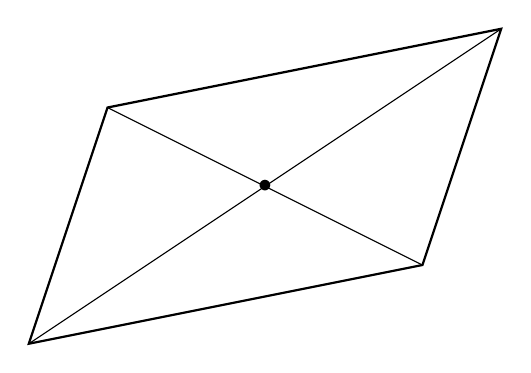
\begin{tikzpicture} [remember picture]
\draw (-3,-2)--(3,2) (-2,1)--(2,-1);
\draw[thick] (-3,-2)--(2,-1)--(3,2)--(-2,1)--cycle;
\node (centre) at (0,0){$\bullet$};  % centre du parallelogramme
\node (parallelogramme) at (-2,1){}; % sommet du parallelogramme
\end{tikzpicture}
\end{center}

Ce point \tikz[remember picture]\coordinate(point); est le milieu des diagonales de ce parall\`elogramme.
% les fleches
\begin{tikzpicture}[remember picture,overlay]
  \draw [->] (figure) to[bend right,thick] (parallelogramme);
  \draw [->] (point) to[bend left,thick,dashed] (centre);
\end{tikzpicture}
\end{minipage}}

\begin{tikzpicture}[remember picture,overlay]
\node [rotate=60,scale=10,text opacity=0.3]
    at (current page.center) {Ti\textit{k}Z};
\end{tikzpicture}

\end{document}
